\titledquestion{Maximum area rectangle in histogram}

We are given a histogram consisting of $n$ parallel bars side by side, each of width $1$, as well as a sequence $A$ containing the heights of the bars where the height of the $i$th bar is $\mathbf{a}_i$ for $\forall \; i \in [n]$. For example, the figures below show the case where $n= 7$ and $A = \langle 6, 2, 5, 4, 4, 1, 3 \rangle$. Our goal is to find the maximum area of the rectangle placed inside the boundary of the given histogram with a \textbf{divide-and-conquer} algorithm. (Here you don't need to find which rectangle maximizes its area.)

Reminder: There do exist algorithms that solve this problem in linear time. However, you are \textbf{not allowed} to use them in this homework. Any other type of algorithms except the divide-and-conquer ones will get \textbf{no} credit.

\begin{figure}[htbp]
    \centering
    \begin{minipage}[t]{0.48\textwidth}
        \centering
        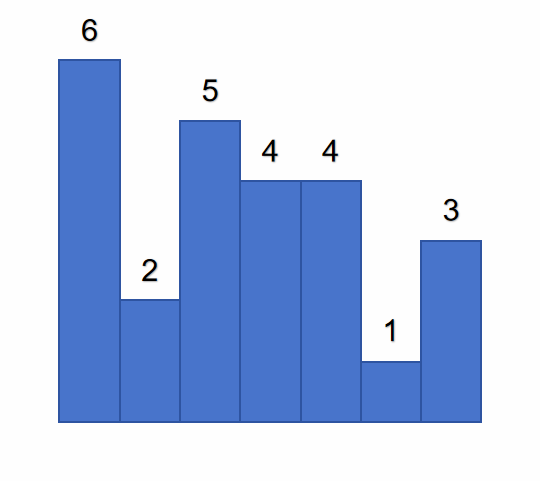
\includegraphics[width=6cm]{withnum.png}
        \caption{The Original Histogram}
    \end{minipage}
    \begin{minipage}[t]{0.48\textwidth}
        \centering
        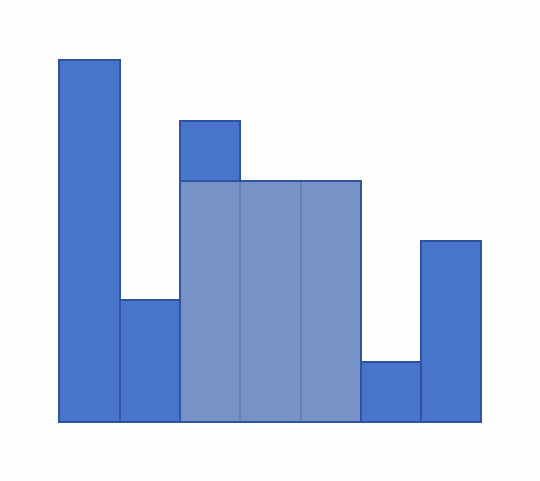
\includegraphics[width=6cm]{withrect.png}
        \caption{The Largest Rectangle in Histogram}
    \end{minipage}
\end{figure}

You may use $Rect(l, r, A)$ to represent the answer of the sub-problem w.r.t. the range $\left[l, r\right]$.

\begin{parts}
    \part[3] \textbf{Briefly} describe:
    \begin{enumerate}
        \item How would you divide the original problem into 2 sub-problems?
        \item Under what circumstances will the answer to the original problem not be covered by the answers of the 2 sub-problems?
        \item Given the answers of the 2 sub-problems, how would you get the answer of the original problem?
    \end{enumerate}
    
    \begin{solution}
    %%%%%%%%%%%%%%%%%%%%%%%%%%%%%%%%%%%%%%%%%%%%%%%%%
    % Replace `\vspace{2in}' with your answer.
    \\
    1.Find the shortest bar(or bars) in the histogram and set its index as smallestbar, and then calculate the maximum rectangular area of the two small histograms around the shortest bars by using Rect(l,smallestbar-1,A) and Rect(smallestbar+1,r,A).\\
    the sub-problem is calculating the largest rectangular area of the two part histograms around the shortest bars.\\
    2.When the area enclosed by the shortest bar(including the area enclosed by the left and right small histograms) is larger than the area of the largest rectangular area in the left and right small histograms, the answer to the original problem not be covered by the answers of the 2 sub-problems.\\
    3.Compare the area of the largest rectangle from the smallest histogram until the area of the larger of the two smaller histograms in the largest histogram is obtained, and compared with the area surrounded by the shortest bar, and then the larger one is the answer of the original problem.\\
    %%%%%%%%%%%%%%%%%%%%%%%%%%%%%%%%%%%%%%%%%%%%%%%%%
    \end{solution}

    \newpage
    
    \part[8] Based on your idea in part(a), design a \textbf{divide-and-conquer} algorithm for this problem. Make sure to provide \textbf{clear description} of your algorithm design in \textbf{natural language}, with \textbf{pseudocode} if necessary.
    
    \begin{solution}
    %%%%%%%%%%%%%%%%%%%%%%%%%%%%%%%%%%%%%%%%%%%%%%%%%
    % Replace `\vspace{7.5in}' with your answer.
    \\
    1.First, we traverse the histogram to find the shortest bar, then calculate the rectangular area surrounded by the shortest bar, and then operate the left and right histograms of the bar to find the largest rectangular area of each, and compare the larger one with the rectangle surrounded by the shortest bar to get the largest rectangular area.\\
    2.Similarly, to find the largest rectangular area of the two histograms, we first find the shortest bar, and then calculate the maximum rectangular area of its circumference, and the maximum rectangular area of the left and right histograms to find the maximum rectangular area between the three.\\
    3.This keeps dividing until the left and right histograms of the shortest bar contain only one bar.\\
    \\
    Pseudocode(maybe it does not satisfies the standard):\\
    \begin{cpp}
    left and right are indices of the left most and rightmost elements in given array arr respectively.\\
    function Rect(A, left, right)
        shortestbar = A[left];
        if right = left then
            return A[left]
        i = left;
        while(i < right)
            if (shortestbar > A[i++]) then
                shortestbar = A[i];
                shortestbarindex = i;
        if i = right then
            return max(shortestbar * (right-left+1), max(Rect(A, left, i-1), Rect(A, i+1, right)))
    \end{cpp}
    %%%%%%%%%%%%%%%%%%%%%%%%%%%%%%%%%%%%%%%%%%%%%%%%%
    \end{solution}

    \newpage
    
    \part[2] Provide the run-time complexity analysis of your algorithm in part (b). Make sure to include the \textbf{recurrence relation} of the run-time in your solution.
    
    \begin{solution}
    %%%%%%%%%%%%%%%%%%%%%%%%%%%%%%%%%%%%%%%%%%%%%%%%%
    % Replace `\vspace{3in}' with your answer.
    \\
    For the average case is that each sub-histogram can be divided constantly and be divided int a bar at the same level.\\
    On the zero level, we traverse the histogram and find the smallest bar which spend $\theta(n)$ time. And calculating the rectangle surrounded by the smallest bar and comparing the left and right indices spends constant time.\\
    And then we recursively divide the histogram into two smaller histograms by the smallest bar.\\
    For each smaller histogram, we spend the same proportion of time as the length of this histogram over the length of the larger histogram to traverse but all the total length of all histograms is approxiately the length of the histogram before it was divided.So on the next level, we spend the same time as before on the searching for the smallest bar. i.e. the work on the following level(all) is $\theta(n)$.\\
    Then for the average case, we get the recursive tree is that:\\
    Which recursive function is $T(n) = aT(\frac{n}{b}) + \theta(n)$ where a and b can be approximated as 2(for average).\\
    branching factor a,    the problem size is $\frac{n}{b^{k}}$ on the kth level and the work is $a^{k}(\frac{n}{b}^{k})^{d=1} = n$,  the levels is $logn$.\\
    Then the total time complexity of the algorithm is $\sum_{1}^{logn}a^{k}(\frac{n}{b^{k}}) = nlogn$.\\
    i.e. O(nlog(n))\\
    \\
    \\
    of course, if the histogram is an ascending or descending order, we can't divide it equally but one by one, then it's the worst case that we should do $\sum_{i=1}^{n}i$ = $\frac{n^{2}-n}{2}$ whose time complexity is $O(n^{2})$
    %%%%%%%%%%%%%%%%%%%%%%%%%%%%%%%%%%%%%%%%%%%%%%%%%
    \end{solution}
    
\end{parts}